\documentclass[11pt]{article}
\usepackage[margin=1in]{geometry}
\usepackage{amsmath,amssymb,amsthm}
\usepackage{graphicx}
\usepackage{hyperref}

\newtheorem{theorem}{Theorem}
\newtheorem{lemma}{Lemma}
\newcommand{\R}{\mathbb R}
\newcommand{\Q}{\mathbb Q}
\renewcommand{\O}{\mathbb O}
\newcommand{\Sph}{\mathbb S}
\newcommand{\cR}{\mathcal R}
\newcommand{\cV}{\mathcal V}
\newcommand{\Iso}{\operatorname{Iso}}

\title{The weak octonionic Stiefel space \(V^{\mathrm w}_2(\O^2)\)\\
is not a manifold}
\author{A full negative answer to modified James Question (2) in arXiv:2605.07226}
\date{11 August 2026}

\begin{document}
\maketitle

\noindent\textbf{Status.}
\texttt{candidate\_full\_negative\_answer\_likely\_valid\_needs\_human\_review}.

\begin{abstract}
Huo, Ren, and Xu ask whether their weak octonionic Stiefel spaces
\(V^{\mathrm w}_k(\O^n)\) are manifolds. We give a negative answer in the
smallest nontrivial case: \(V^{\mathrm w}_2(\O^2)\) is not even a topological
manifold. Using the source's classification of this space as the octonionic
isometry locus, we prove that a neighborhood of the identity is homeomorphic
to a neighborhood of the origin in
\[
 \R^8\times
 \{(A,B)\in\R^7\times\R^7:
       \operatorname{rank}[A\ B]\le1\}.
\]
The second factor is the rank-one determinantal cone. Its link is
\((\Sph^6\times\Sph^1)/\{\pm1\}\), which has nonzero rational first
homology. The resulting local homology is incompatible with a
\(16\)-manifold.
\end{abstract}

\section{Source question and imported classification}

A finite family \((x_1,\ldots,x_k)\) in \(\O^n\) is a weak associative
orthonormal set when it is orthonormal and
\[
 \langle p x_i,x_j\rangle-p\langle x_i,x_j\rangle=0
 \qquad(p\in\O)
\]
for every \(i,j\). The source defines
\[
 V^{\mathrm w}_k(\O^n)
 =\{(x_1,\ldots,x_k):
       (x_1,\ldots,x_k)\text{ is a weak associative orthonormal set}\}
\]
and asks:
\begin{quote}
Is \(V^{\mathrm w}_k(\O^n)\) a manifold?
\end{quote}
See Figure~\ref{fig:question}. Its modified projection question is answered
inside the same paper, but this manifold question is left open.

We use one result from \cite{source}. Regard a pair in
\(V^{\mathrm w}_2(\O^2)\) as the two rows of a \(2\times2\) octonionic
matrix. Source Theorems 3.12 and 3.16 identify
\[
 V^{\mathrm w}_2(\O^2)=\Iso_{\O}(2)
 =\bigcup_{J\in\Sph^6} \Sph^7 U_{\mathbb C_J}(2),
 \qquad \mathbb C_J=\R\oplus\R J.
\]
Equivalently, every such matrix is \(pU\) for a unit octonion \(p\) and
a unitary \(2\times2\) matrix \(U\) over some complex slice
\(\mathbb C_J\); see Figure~\ref{fig:classification}.

\section{Proof intuition}

Near the identity, the upper-left entry is nonzero. Dividing out its unit
octonionic phase uniquely separates seven ordinary spherical directions.
The remaining normalized matrix is complex-unitary in some slice
\(\mathbb C_J\) and has positive-real upper-left entry.

Such a unitary matrix has one real off-diagonal coordinate \(s\), while its
two imaginary parameters \(A\) and \(B\) must point in the same imaginary
octonionic direction \(J\). Thus the singular part of the local model is
exactly the variety of collinear pairs in \(\R^7\), or equivalently the
\(7\times2\) matrices of rank at most one. At the cone vertex, the direction
\(J\) is undefined. The link remembers this collapse and has extra first
homology, preventing local Euclidean structure.

\section{The local normal form}

Put
\[
 \cR=\{(A,B)\in\R^7\times\R^7:
             A\wedge B=0\}
     =\{(A,B):\operatorname{rank}[A\ B]\le1\}.
\]
We identify \(\R^7\) with the imaginary octonions.

\begin{lemma}[Local determinantal chart]\label{lem:chart}
Let \(I\) be the identity matrix in \(V^{\mathrm w}_2(\O^2)\). A
neighborhood of \(I\) is homeomorphic, as a pointed space, to a neighborhood
of \(0\) in \(\R^8\times\cR\).
\end{lemma}

\begin{proof}
Write a matrix near \(I\) as
\[
 M=\begin{pmatrix}a&b\\c&d\end{pmatrix}.
\]
Its upper-left entry \(a\) is nonzero. Define
\[
 p=\frac a{|a|}\in\Sph^7,
 \qquad U=\overline p,M,
\]
where \(\overline p\) multiplies every entry on the left. The proof of source
Theorem 3.16 shows that \(U\in U_{\mathbb C_J}(2)\) for some \(J\), and its
upper-left entry is \(|a|>0\). Conversely, \(pU\) is in the weak Stiefel
space for every such pair. This normalization is unique, continuous, and has
continuous inverse: the upper-left entry of \(pU\) is \(p r\) with
\(r>0\), so it recovers \(p\). Hence the germ splits as a neighborhood of
\(1\) in \(\Sph^7\) times the germ of normalized matrices \(U\).

We now parametrize the normalized germ. A complex unitary matrix near
\(I\), with positive-real upper-left entry, has the unique form
\begin{equation}\label{eq:unitary-form}
 U=
 \begin{pmatrix}
  r&s+B\\
  -e^A(s-B)&e^A r
 \end{pmatrix},
 \qquad
 r=\sqrt{1-s^2-|B|^2},
\end{equation}
where \(s\in\R\) is small and \(A,B\in\R J\) for the same imaginary unit
\(J\). Indeed, the first row is \((r,z)\), with \(z=s+B\), and every unit
row orthogonal to it is
\(e^A(-\overline z,r)\), for a unique unit complex phase \(e^A\) near one.

The condition that \(A\) and \(B\) belong to one line \(\R J\) is precisely
\((A,B)\in\cR\). Formula~\eqref{eq:unitary-form} is independent of a choice
of \(J\) when one or both vectors vanish. Conversely, from \(U\) one
recovers
\[
 s=\operatorname{Re}U_{12},\qquad
 B=\operatorname{Im}U_{12},\qquad
 A=\log(U_{22}/r),
\]
using the unique logarithm near one. Thus the normalized germ is
homeomorphic to the germ of \(\R\times\cR\). Finally, a neighborhood in
\(\Sph^7\) is \(\R^7\), giving
\[
 (\Iso_{\O}(2),I)\cong(\R^7\times\R\times\cR,0).
\]
\end{proof}

\section{The homology obstruction}

\begin{theorem}\label{thm:not-manifold}
The space \(V^{\mathrm w}_2(\O^2)\) is not a topological manifold.
Consequently modified James Question (2) in \cite{source} has a negative
answer in general.
\end{theorem}

\begin{proof}
The determinantal variety \(\cR\) is the cone on its unit link
\[
 L=\cR\cap\Sph^{13}
   \cong(\Sph^6\times\Sph^1)/\sim,
 \qquad (u,v)\sim(-u,-v).
\]
Indeed, every nonzero rank-one \(7\times2\) matrix of Frobenius norm one has
a factorization \(uv^{\mathsf T}\) with \(u\in\Sph^6\) and
\(v\in\Sph^1\), unique up to simultaneous sign.

The displayed quotient is a two-sheeted cover. With rational coefficients,
transfer identifies its homology with the invariant part of
\(H_*(\Sph^6\times\Sph^1;\Q)\). The deck transformation is antipodal on
both factors. On \(H_1(\Sph^1;\Q)\) it is rotation by \(\pi\), hence has
degree \(+1\). Therefore
\begin{equation}\label{eq:h1}
 H_1(L;\Q)\cong\Q.
\end{equation}

At a nonzero rank-one point, \(\cR\) is a smooth determinantal variety of
dimension
\[
 1(7+2-1)=8.
\]
Lemma~\ref{lem:chart} therefore gives nearby smooth points of local
dimension \(8+8=16\). If a neighborhood of \(I\) were a manifold, its
dimension would be \(16\).

For the pointed local model \(X=\R^8\times C(L)\), the local Kunneth
formula and the cone formula give
\[
 H_k(X,X\setminus\{0\};\Q)
 \cong \widetilde H_{k-9}(L;\Q).
\]
By \eqref{eq:h1}, the local homology group in degree \(k=10\) is nonzero.
A topological \(16\)-manifold has local rational homology only in degree
\(16\). Hence the identity is not locally Euclidean, proving the claim.
\end{proof}

\section{Verification, novelty, and scope}

The exact checker verifies \(21{,}000\) rank-one minors and
\(60{,}000\) rational complex-unitary and recovery identities, including exact recovery
of the parameters in \eqref{eq:unitary-form}. These computations guard
against coordinate and sign errors but do not replace the topological proof.

Four lightweight run indexes and bounded exact-title, weak-Stiefel, and
octonionic-manifold searches found no duplicate or later resolution through
11 August 2026. The result answers the source's general yes/no question
negatively via \((k,n)=(2,2)\). It does not classify which other pairs
\((k,n)\) may yield manifolds. Human review should focus on the uniqueness
of the top-left normalization, the local parametrization
\eqref{eq:unitary-form}, and the local-homology degree shift.

\begin{thebibliography}{9}
\raggedright
\bibitem{source}
Q. Huo, G. Ren, and Z. Xu,
\emph{Octonionic isometric isomorphisms and partial isometry},
arXiv:2605.07226 (2026), Theorems 3.12 and 3.16 and Section 4.
\end{thebibliography}

\begin{figure}[ht]
\centering

\includegraphics[width=0.95\textwidth]{figures/source_question.png}
\caption{Source PDF page 23: the modified James questions, including whether
\(V^{\mathrm w}_k(\O^n)\) is a manifold.}
\label{fig:question}
\end{figure}

\begin{figure}[ht]
\centering
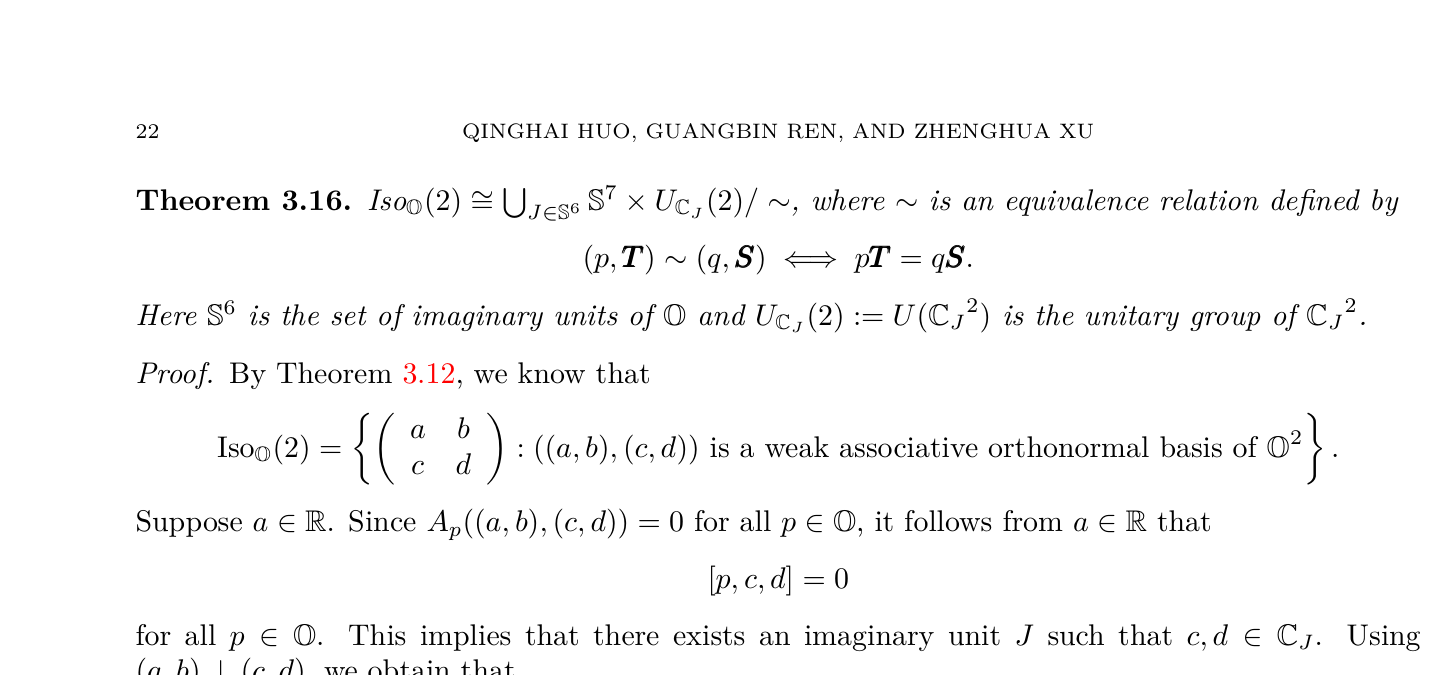
\includegraphics[width=0.95\textwidth]{figures/source_classification.png}
\caption{Source PDF page 22: the \(2\times2\) octonionic isometry
classification used in the local chart.}
\label{fig:classification}
\end{figure}

\end{document}
